\section{Special Execution Platforms}
\label{sec:Execution_Platfors}

This section provides information about how to run COMPSs Applications in specific platforms such as \textit{Docker},
\textit{Chameleon} or \textit{MareNostrum}.


%%%%%%%%%%%%%%%%%%%%%%%%%%%%%%%%%%%%%%%%%
%% DOCKERS
%%%%%%%%%%%%%%%%%%%%%%%%%%%%%%%%%%%%%%%%%
\subsection{Docker}

\subsubsection{Introduction}
Docker is an open-source project that automates the deployment of applications inside software containers, 
by providing an additional layer of abstraction and automation of operating-system-level virtualization on Linux.
In addition to the Docker container engine, there are other Docker tools that allow users to create complex applications (Docker-Compose) 
or to manage a cluster of Docker containers (Docker Swarm).
\\ \\ 
COMPSs supports running a distributed application in a Docker swarm cluster.
\\

\subsubsection{Requirements}
In order to use COMPSs with Docker, some requirements must be fulfilled:
\begin{itemize}  
\item Have \textbf{Docker} and \textbf{Docker-Compose} installed in your local machine.
\item Have an available \textbf{Docker swarm cluster} and its swarm manager ip and port to access it remotely.
\item A \textbf{Dockerhub account}. Dockerhub is an online repository for Docker images. We don't currently support
      another sharing method besides uploading to Dockerhub, so you will need to provide a username.
      This has the advantage that it takes very little to upload the image, since Dockerhub 
      will just need the delta layers from the base image of COMPSs.
\end{itemize}

For more information about Docker and how to install different components, visit Docker site: \url{https://www.docker.com/}

\clearpage
\subsubsection{Execution}
To execute COMPSs in a Docker swarm cluster, you must use the \textbf{runcompss-docker} command, instead of runcompss.
\\
The command \textbf{runcompss-docker} has some \textbf{additional arguments} that will be needed by COMPSs to run your application 
in a distributed Docker swarm cluster environment.
The rest of typical arguments (classpath, project, etc.) will be delegated to runcompss command.
\\ \\
These \textbf{mandatory} additional arguments must go \textbf{before} the typical runcompss arguments. 
The \textbf{runcompss-docker additional arguments} are:
\begin{itemize}
 \item { 
 \textbf{-{}-w, -{}-worker-containers:} \\  
 Specifies the number of \textbf{worker containers} the app will execute on. One more container will be created to host the \textbf{master}. 
 If you have enough nodes in the swarm cluster, each container will be executed by one node.\\
 Example:  \textbf{-{}-worker-containers=3}
 }
 
 \item { 
 \textbf{-{}-c, -{}-context-dir:} \\
 Specifies the \textbf{context directory} of the app. 
 The context directory is a local directory that \textbf{must contain the needed binaries and input files of the app}.
 In its simplest case, it will contain the executable file (a .jar for example).
 Take into account that you should not put unnecessary files in the context-directory, 
 since \textbf{it will be copied to all the nodes} that need it.
 
 Example: \textbf{-{}-context-dir='/home/compss-user/my-app-dir'}, where my-app-dir contains 'app.jar', 'data1.dat' and 'data2.csv', for example.
 }

 \item { 
 \textbf{-{}-s, -{}-swarm-manager:} \\
 Specifies the swarm manager ip and port (format: <ip>:<port>). 
 You can test if the swarm manager really works and is reachable from your machine
 running from your machine the Docker hello-world container.\\
 Example: \textbf{-{}-swarm-manager='129.114.108.8:4000'}
 }
 
 \item { 
 \textbf{-{}-u, -{}-username:} \\
 Specifies a \textbf{Dockerhub username}, to upload the app image, so the workers can pull it in runtime. 
 As stated in the requirements sections, this is needed to share your container application image with the nodes that need it.
 }
\end{itemize}

As an \textbf{optional} argument:
\begin{itemize}
 \item { 
 \textbf{-{}-n, -{}-no-refresh-app-image:} \\
 If this flag is on, the \textbf{app image won't be uploaded }to Dockerhub.
 Workers won't pull the image either.
 Use this flag if the application has not changed since the last running.
 This way the execution will be \textbf{faster}, and you won't need to specify the Dockerhub username nor write its password.
 But remember! If you make any change to the application, run an execution without this flag at least once, 
 to update the online application image.
 }
\end{itemize}

Here is the \textbf{format} you must use with \textbf{runcompss-docker} command:
\begin{lstlisting}[language=bash]
runcompss-docker --worker-containers=N 
                 --context-dir='CTX_DIR'
                 --swarm-manager='<ip>:<port>'
                 --username='dockerhub_username'
                 [rest of classic runcompss args]
\end{lstlisting}           

Or alternatively, in its shortest form:
\begin{lstlisting}[language=bash]
runcompss-docker --w=N  --c='CTX_DIR' --s='<ip>:<port>' --u='dockerhub_username' 
                 [rest of classic runcompss args]
\end{lstlisting}        

The runcompss-docker command creates a Docker image from a common COMPSs docker image by adding your context directory to it. 
Then it uploads this image to Dockerhub and Docker Compose is in charge of spawning the different application containers to the docker swarm manager.
Then the Docker Swarm starts the containers and the application.
\\
The COMPSs Docker base image is available in the Dockerhub. In case you need it, you can pull it using the following command:
\begin{lstlisting}[language=bash]
docker pull compss/compss
\end{lstlisting}

\clearpage
\subsubsection{Execution with TLS}
If your cluster uses \textbf{TLS} or has been created using \textbf{Docker-Machine}, you will have to 
\textbf{export two environment variables} before using runcompss-docker:\\ \\
On one hand, \textbf{DOCKER\_TLS\_VERIFY} environment variable will tell Docker that you are using TLS:
\begin{lstlisting}[language=bash]
export DOCKER_TLS_VERIFY="1"
\end{lstlisting}
On the other hand, \textbf{DOCKER\_CERT\_PATH} variable will tell Docker where to find your TLS certificates. As an example:
\begin{lstlisting}[language=bash]
export DOCKER_CERT_PATH="/home/compss-user/.docker/machine/machines/my-manager-node"
\end{lstlisting}

In case you have created your cluster using docker-machine, in order to know what
your \textit{DOCKER\_CERT\_PATH} is, you can use this command:
\begin{lstlisting}[language=bash]
docker-machine env my-swarm-manager-node-name | grep DOCKER_CERT_PATH
\end{lstlisting}
In which \textit{swarm-manager-node-name} must be changed by the name docker-machine has assigned to your swarm manager node.\\ \\
With these environment variables set, you are ready to use \textbf{runcompss-docker} in a cluster using TLS.

\clearpage
\subsubsection{Execution results}
The execution results will be retrieved from the master container of your application.
\\ \\ 
If your context-directory name is \textbf{'matmul'}, then your results will be saved in the \textbf{'matmul-results'} directory, 
which \textbf{is located in the SAME directory as your context-directory is in}. 
\\ \\ 
Inside the \textbf{'matmul-results'} directory you will have:
\begin{itemize}
 \item  A folder named \textbf{'matmul'} with all the result files that were
	in the same directory as the executable when the application execution ended.  
	More precisely, this will contain the context-directory state right after finishing your application execution.
	\\
	\\
	Additionally, and for more advanced debug purposes,
	you will have some intermidiate files created by runcompss-docker(Dockerfile, project.xml, resources.xml),
	in case you want to check for more complex errors or details. 
	
	
  \item A folder named \textbf{'debug'}, which (in case you used the runcompss debug option (\textbf{-d})), 
        will contain the \textbf{'.COMPSs'} directory, which contains another directory in which there are the typical debug files runtime.log, jobs, etc.
	\\
        Remember \textbf{.COMPSs} is a \textbf{hidden} directory, take this into account if you do \textbf{ls} inside the debug directory (add the \textbf{-a} option).
  
\end{itemize}

To make it simpler, we provide a \textbf{tree visualization} of an example of what your directories should look like after the execution.
In this case we executed the \textbf{Matmul example application} that we provide you:
\\*
\\*
\\*
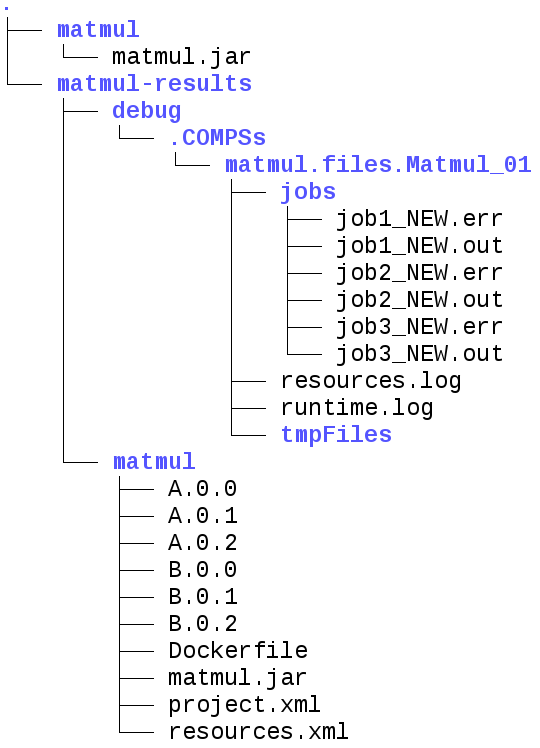
\includegraphics[width=0.3\textwidth]{./Sections/5_Execution_Platforms/Figures/docker-matmul-results-tree.png} 

\clearpage
\subsubsection{Execution examples}
And here is one example to run the Matmul example application. 
In this case, we are specifying:

\begin{itemize}  
\item Use \textbf{5 worker docker containers}. They will be distributed amongst the swarm cluster nodes as balanced as possible.
\item The \textbf{context directory} will be '/home/compss-user/my-app-dir'.
\item The \textbf{swarm-manager ip} will be 129.114.108.8, with the swarm manager located in the \textbf{port} 4000.
\item The \textbf{Dockerhub username} will be john123 (the \textbf{password} will be asked when executing runcompss-docker).
\item The \textbf{classpath} will be '/home/compss-user-john/matmul/matmul.jar', and we will use \textbf{debug (-d)}.
\item Finally, as we would do with the typical runcompss, we specify the \textbf{main class} name and its \textbf{parameters} (16 and 4 in this case).
\end{itemize}
And this is how you would run \textbf{runcompss-docker}:
\begin{lstlisting}[language=bash]
runcompss-docker --worker-containers=5 \
                 --context-dir='/home/compss-user/my-app-dir' \
                 --swarm-manager='129.114.108.8:4000' \
                 --username='john123' \
                 --classpath=/home/compss-user/my-app-dir/my-app.jar \
                 -d \
                 matmul.objects.Matmul 16 4
\end{lstlisting}           

Here we show another example using the short arguments form, with the KMeans example application, that we provide to you:
\begin{lstlisting}[language=bash]
runcompss-docker --w=30 --c='./kmeans-app' --s='110.3.14.159:26535' --u='test1947' \
                 --classpath=./kmeans/kmeans.jar \
                 kmeans.KMeans
\end{lstlisting}           



\clearpage

%%%%%%%%%%%%%%%%%%%%%%%%%%%%%%%%%%%%%%%%%
%% CHAMEMELON
%%%%%%%%%%%%%%%%%%%%%%%%%%%%%%%%%%%%%%%%%
\subsection{Chameleon}

\subsubsection{Introduction}

The Chameleon project is a configurable experimental environment for large-scale cloud research based on a \textit{OpenStack} 
KVM Cloud. With funding from the \textit{National Science Foundation (NSF)}, it provides a large-scale platform to the open research
community allowing them explore transformative concepts in deeply programmable cloud services, design, and core technologies. The 
Chameleon testbed, is deployed at the \textit{University of Chicago} and the \textit{Texas Advanced Computing Center} and consists of
650 multi-core cloud nodes, 5PB of total disk space, and leverage 100 Gbps connection between the sites. 

The project is led by the \textit{Computation Institute} at the \textit{University of Chicago} and partners from the \textit{Texas 
Advanced Computing Center} at the \textit{University of Texas} at Austin, the \textit{International Center for Advanced Internet 
Research} at \textit{Northwestern University}, the \textit{Ohio State University}, and \textit{University of Texas} at \textit{San
Antoni}, comprising a highly qualified and experienced team. The team includes members from the \textit{NSF} supported 
\textit{FutureGrid} project and from the \textit{GENI} community, both forerunners of the \textit{NSFCloud} solicitation under 
which this project is funded. Chameleon will also sets of partnerships with commercial and academic clouds, such as \textit{Rackspace},
\textit{CERN} and \textit{Open Science Data Cloud (OSDC)}.

For more information please check \url{https://www.chameleoncloud.org/} .

\subsubsection{Execution}
Currently, COMPSs can only handle the Chameleon infrastructure as a cluster (deployed inside a lease). Next, we provide the steps
needed to execute COMPSs applications at Chameleon:

\begin{itemize}
 \item Make a lease reservation with 1 minimum node (for the COMPSs master instance) and a maximum number of nodes equal to the
 number of COMPSs workers needed plus one
 \item Instantiate the master image (based on the published image \textit{COMPSs\_\compssversion\_CC-CentOS7})
 \item Attach a public IP and login to the master instance (the instance is correctly contextualized for COMPSs executions if you
 see a COMPSs login banner)
 \item Set the instance as COMPSs master by running \textit{/etc/init.d/chameleon\_init start}
 \item Copy your CH file (API credentials) to the Master and source it
 \item Run the \textit{chameleon\_cluster\_setup} script and fill the information when prompted (you will be asked for the name of the
 master instance, the reservation id and number of workers). This scripts may take several minutes since it sets up the all cluster.
 \item Execute your COMPSs applications normally using the \textit{runcompss} script
\end{itemize}

As an example you can check this video \url{https://www.youtube.com/watch?v=BrQ6anPHjAU} performing a full setup and 
execution of a COMPSs application at Chameleon.


%%%%%%%%%%%%%%%%%%%%%%%%%%%%%%%%%%%%%%%%%
%% SuperComputers
%%%%%%%%%%%%%%%%%%%%%%%%%%%%%%%%%%%%%%%%%
\subsection{SuperComputers}

To maintain the portability between different environments, COMPSs has a pre-build structure (see Figure 
\ref{fig:queue_scripts_structure}) to execute applications in SuperComputers. For this purpose, users must use 
the \textit{enqueue\_compss} script provided in the COMPSs installation. This script has several parameters (see 
\textit{enqueue\_compss -h}) that allow users to customize their executions for any SuperComputer.

\begin{figure}[h!]
  \centering
    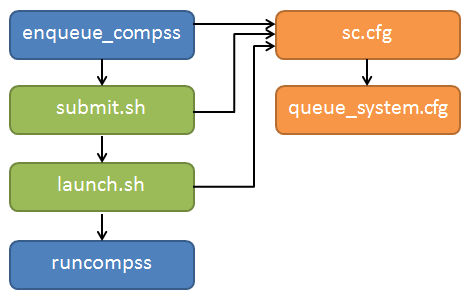
\includegraphics[width=0.6\textwidth]{./Sections/5_Execution_Platforms/Figures/queue_scripts_structure.png}
    \caption{Structure of COMPSs queue scripts. In Blue user scripts, in Green queue scripts and in Orange system dependant scripts}
    \label{fig:queue_scripts_structure}
\end{figure}

To make this structure works, the administrators must define a configuration file for the queue system and a configuration file
for the specific SuperComputer parameters. The COMPSs installation already provides queue configurations for \textit{LSF} and 
\textit{SLURM} and several examples for SuperComputer configurations. 
To create a new configuration we recommend to use one of the configurations provided by COMPSs (such as the configuration for the
\textit{MareNostrum III} SuperComputer) or to contact us at \url{support-compss@bsc.es} .

\subsubsection{MareNostrum III}

For information about how to submit COMPSs applications at MareNostrum III (BSC) please refer to the \textit{COMPSs at BSC} manual 
available at \url{http://compss.bsc.es/releases/compss/latest/docs/COMPSs_MareNostrum_Manual.pdf} .
